%%
% The BIThesis Template for Bachelor Graduation Thesis
%
% 北京理工大学毕业设计(论文) —— 使用 XeLaTeX 编译
%
% Copyright 2021 BITNP
%
% This work may be distributed and/or modified under the
% conditions of the LaTeX Project Public License, either version 1.3
% of this license or (at your option) any later version.
% The latest version of this license is in
%   http://www.latex-project.org/lppl.txt
% and version 1.3 or later is part of all distributions of LaTeX
% version 2005/12/01 or later.
%
% This work has the LPPL maintenance status `maintained'.
%
% The Current Maintainer of this work is Feng Kaiyu.
%
% Compile with: xelatex -> biber -> xelatex -> xelatex

% 章节支持、单面打印:ctexbook
\documentclass[bachelor,footskip=24pt]{bitbook}
% 如果想要修改样式,但无法找到样式在哪里定义:请参考 https://bithesis.bitnp.net/Guide/4-Others/Troubleshooting.html#%E6%83%B3%E8%A6%81%E4%BF%AE%E6%94%B9%E9%83%A8%E5%88%86%E6%A0%B7%E5%BC%8F-%E4%BD%86%E6%98%AF%E6%89%BE%E4%B8%8D%E5%88%B0%E6%A0%B7%E5%BC%8F%E5%9C%A8%E5%93%AA%E9%87%8C%E5%AE%9A%E4%B9%89

% 另一个临时的“修改页眉文字”的解决方法(非常不优雅,只作为临时措施)。
% 请注释掉以下 20 行内容使用。
% % 从原有主题继承自定义主题
% \fancypagestyle{BIThesisCustom}[BIThesis]{
%   % 定义页眉、页码
%   \fancyhead[C]{\zihao{4}\ziju{0.08}\songti{北京理工大学本科生毕业设计(论文)覆盖}}
% }
% % 设置章节格式
% \ctexset{chapter={
%     pagestyle = BIThesisCustom,
%   }
% }
% % 前置页面(原创性声明、中英文摘要、目录等)
% \renewcommand{\frontmatter}{
%   \pagenumbering{Roman}
%   \pagestyle{BIThesisCustom}
% }
% % 正文页面
% \renewcommand{\mainmatter}{
%   \pagenumbering{arabic}
%   \pagestyle{BIThesisCustom}
% }
% ------------------------------------------------------------------

% 使用 listings 宏包进行代码块使用,并使用了预定义的样式,
% 你也可以选用自己的喜欢的其他宏包,如 minted;
% 然而由于 minted 依赖 Python 的 Pygments 库作为外部依赖,因此出于模板的建议性考虑,我们没有提供 minted 进行代码块书写的示例。
% 但是,我们仍旧非常建议你使用 minted。
\usepackage{listings}
\usepackage{hyperref}


% 参考文献引用文件位于 misc/ref.bib
\addbibresource{misc/ref.bib}

% 在这里填写你的论文中英文题目
\newcommand{\thesisTitle}{代理内核操作系统实验PKE在K210开发板上的移植和改进}
\newcommand{\thesisTitleEN}{Transplantation and improvement of Proxy Kernel operating system experiment (PKE) on K210 board}


% 在这里填写你的相关信息
\newcommand{\deptName}{计算机学院}
\newcommand{\majorName}{计算机科学与技术}
\newcommand{\yourName}{张国安}
\newcommand{\yourStudentID}{1120181447}
\newcommand{\mentorName}{陆慧梅}
% 如果你的毕设为校外毕设,请将下面这一行语句解除注释(删除第一个百分号字符)并在第二组花括号中填写你的校外毕设导师名字
% \newcommand{\externalMentorName}{左偏树}

% 文档开始
\begin{document}

% 标题页面:如无特殊需要,本部分无需改动
%%
% The BIThesis Template for Bachelor Graduation Thesis
%
% 北京理工大学毕业设计(论文)封面页 —— 使用 XeLaTeX 编译
%
% Copyright 2020-2021 BITNP
%
% This work may be distributed and/or modified under the
% conditions of the LaTeX Project Public License, either version 1.3
% of this license or (at your option) any later version.
% The latest version of this license is in
%   http://www.latex-project.org/lppl.txt
% and version 1.3 or later is part of all distributions of LaTeX
% version 2005/12/01 or later.
%
% This work has the LPPL maintenance status `maintained'.
%
% The Current Maintainer of this work is Feng Kaiyu.
%
% 封面
%
% 如无特殊需要,本页面无需更改

% Underline new command for student information
% Usage: \dunderline[<offset>]{<line_thickness>}
\newcommand\dunderline[3][-1pt]{{%
  \setbox0=\hbox{#3}
  \ooalign{\copy0\cr\rule[\dimexpr#1-#2\relax]{\wd0}{#2}}}}

% Cover Page
\begin{titlepage}
  \makeatletter
  \@ifundefined{externalMentorName}{
    % 校内毕设封面顶部间距
    \vspace*{19mm}
  }{
    % 校外毕设封面顶部间距
    \vspace*{13mm}
  }
  \centering

  
\includegraphics[width=9.87cm]{images/header.png}

  \vspace*{-3mm}

  \zihao{-0}\textbf{\ziju{0.12}\songti{本科生毕业设计(论文)}}

  \vspace{16mm}

  \zihao{2}\textbf{\xihei\thesisTitle}

  \vspace{3mm}

  \begin{spacing}{1.2}
    \zihao{3}\selectfont{\textbf{\thesisTitleEN}}
  \end{spacing}

  \vspace{15mm}

  \flushleft

  \makeatletter
  \@ifundefined{externalMentorName}{
    % 生成校内毕设封面字段
    \makeatother
    \begin{spacing}{1.8}
      \hspace{27mm}\songti\zihao{3}\selectfont{学\hspace{11mm}院:\dunderline[-10pt]{1pt}{\makebox[78mm][c]{\deptName}}}

      \hspace{27mm}\songti\zihao{3}\selectfont{专\hspace{11mm}业:\dunderline[-10pt]{1pt}{\makebox[78mm][c]{\majorName}}}

      \hspace{27mm}\songti\zihao{3}\selectfont{学生姓名:\dunderline[-10pt]{1pt}{\makebox[78mm][c]{\yourName}}}

      \hspace{27mm}\songti\zihao{3}\selectfont{学\hspace{11mm}号:\dunderline[-10pt]{1pt}{\makebox[78mm][c]{\yourStudentID}}}

      \hspace{27mm}\songti\zihao{3}\selectfont{指导教师:\dunderline[-10pt]{1pt}{\makebox[78mm][c]{\mentorName}}}
    \end{spacing}
  }{
    % 生成校外毕设封面字段
    \makeatother
    \begin{spacing}{1.8}
      \hspace{19.4mm}\songti\zihao{3}\selectfont{学\hspace{19.6mm}院\hspace{3mm}:\dunderline[-10pt]{1pt}{\makebox[77.4mm][c]{\deptName}}}

      \hspace{19.4mm}\songti\zihao{3}\selectfont{专\hspace{19.6mm}业\hspace{3mm}:\dunderline[-10pt]{1pt}{\makebox[77.4mm][c]{\majorName}}}

      \hspace{19.4mm}\songti\zihao{3}\selectfont{学\hspace{2.8mm}生\hspace{2.8mm}姓\hspace{2.8mm}名\hspace{3mm}:\dunderline[-10pt]{1pt}{\makebox[77.4mm][c]{\yourName}}}

      \hspace{19.4mm}\songti\zihao{3}\selectfont{学\hspace{19.6mm}号\hspace{3mm}:\dunderline[-10pt]{1pt}{\makebox[77.4mm][c]{\yourStudentID}}}

      \hspace{19.4mm}\songti\zihao{3}\selectfont{指\hspace{2.8mm}导\hspace{2.8mm}教\hspace{2.8mm}师\hspace{3mm}:\dunderline[-10pt]{1pt}{\makebox[77.4mm][c]{\mentorName}}}

      \hspace{19.4mm}\songti\zihao{3}\selectfont{校外指导教师:\dunderline[-10pt]{1pt}{\makebox[77.4mm][c]{\externalMentorName}}}
    \end{spacing}
  }

  \vspace*{\fill}
  \centering
  \zihao{3}\ziju{0.5}\songti{\today}
\end{titlepage}


% 前置页面定义
\frontmatter
% 原创性声明:如无特殊需要,本部分无需改动
% 更改为 PDF 页面插入,如需要添加内容,可考虑先用 Word 制作再覆盖 misc/1_originality.pdf
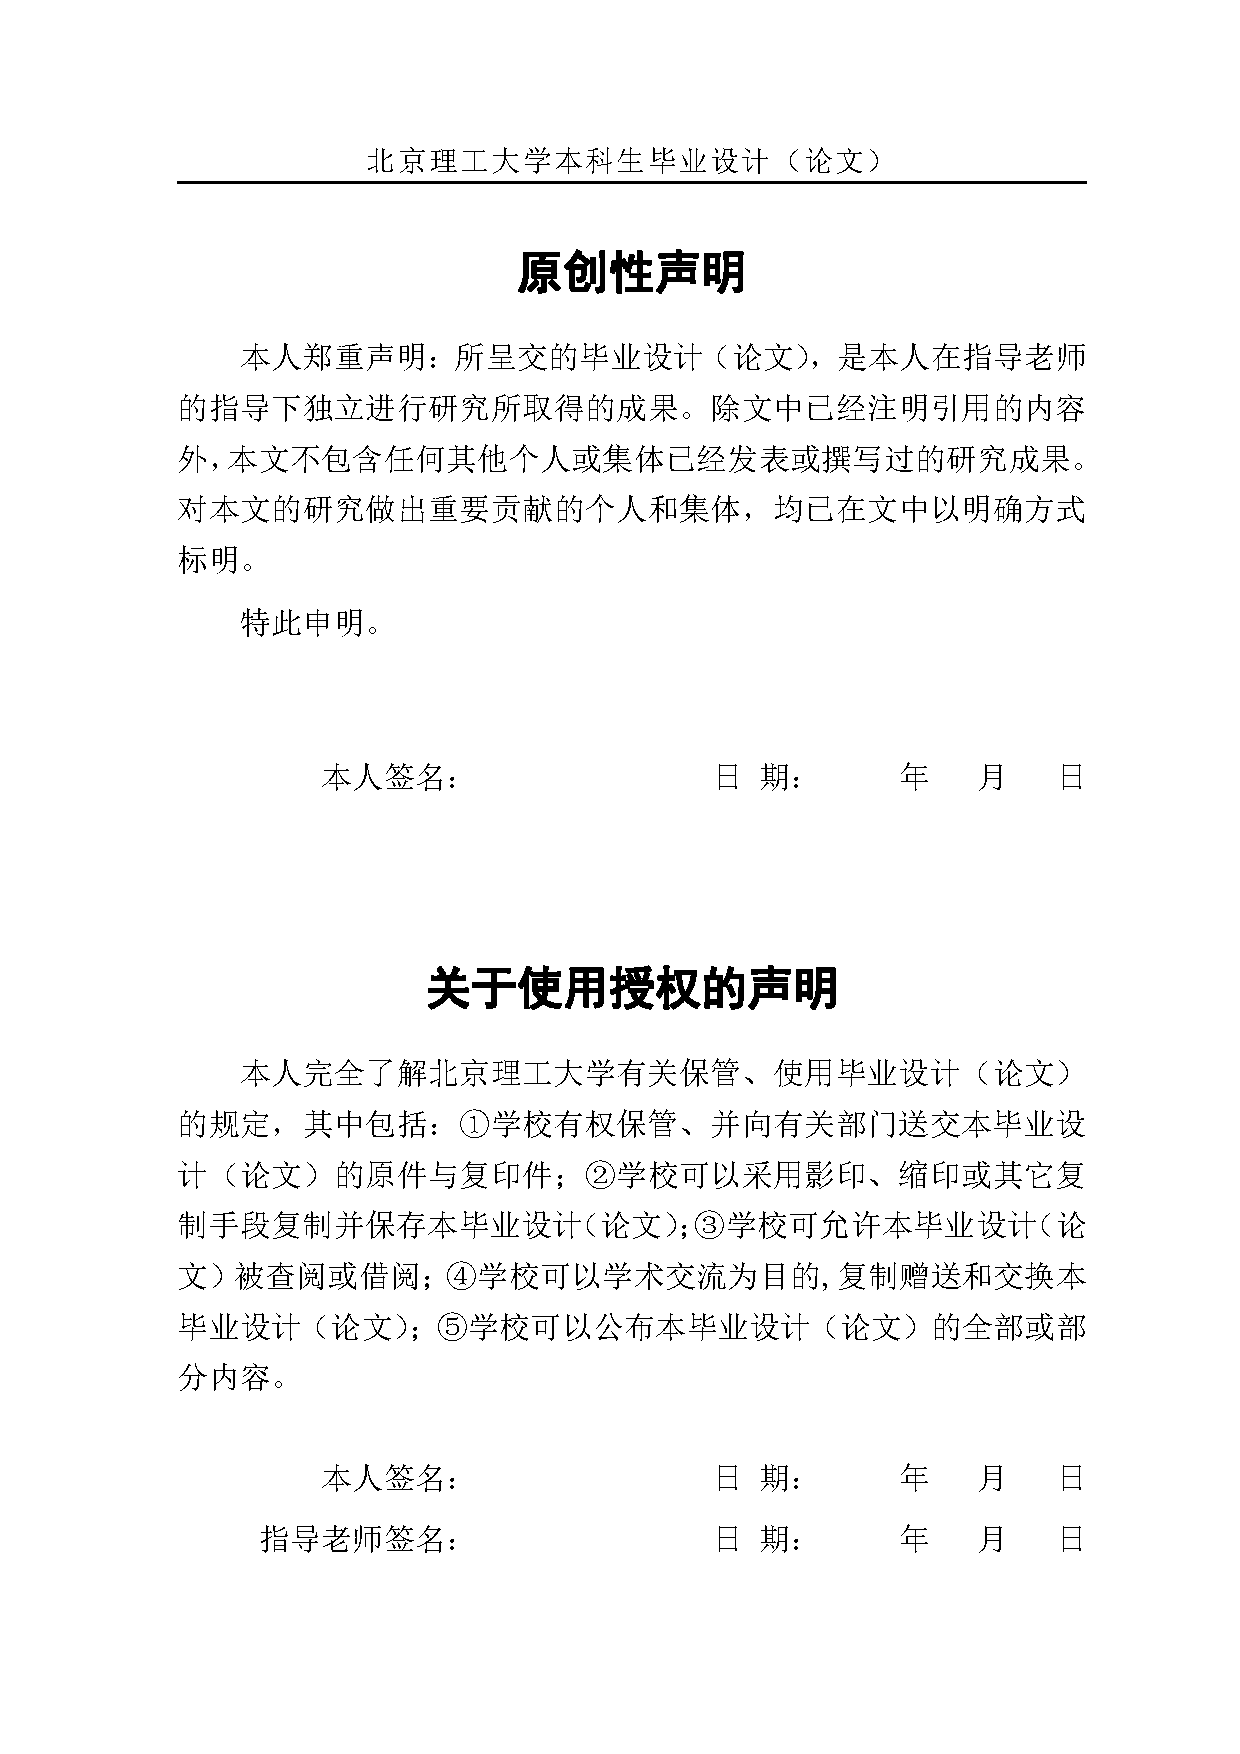
\includepdf{misc/1_originality.pdf}
\newpage
%%%
% The BIThesis Template for Bachelor Graduation Thesis
%
% 北京理工大学毕业设计(论文)原创性声明页 —— 使用 XeLaTeX 编译
%
% Copyright 2020-2021 BITNP
%
% This work may be distributed and/or modified under the
% conditions of the LaTeX Project Public License, either version 1.3
% of this license or (at your option) any later version.
% The latest version of this license is in
%   http://www.latex-project.org/lppl.txt
% and version 1.3 or later is part of all distributions of LaTeX
% version 2005/12/01 or later.
%
% This work has the LPPL maintenance status `maintained'.
%
% The Current Maintainer of this work is Feng Kaiyu.
%
% 如无特殊需要,本页面无需更改

% 原创性声明页无页码页面格式
\fancypagestyle{originality}{
  % 页眉高度
  \setlength{\headheight}{20pt}

  % 页眉和页脚(页码)的格式设定
  \fancyhf{}
  \fancyhead[C]{\zihao{4}\ziju{0.08}\songti{北京理工大学本科生毕业设计(论文)}}

  % 页眉分割线稍微粗一些
  \renewcommand{\headrulewidth}{0.6pt}
}

\pagestyle{originality}
\topskip=0pt

% 圆形数字编号定义
\newcommand{\circled}[2][]{\tikz[baseline=(char.base)]
  {\node[shape = circle, draw, inner sep = 1pt]
  (char) {\phantom{\ifblank{#1}{#2}{#1}}};
  \node at (char.center) {\makebox[0pt][c]{#2}};}}
\robustify{\circled}

% 设置行间距
\setlength{\parskip}{0.4em}
\renewcommand{\baselinestretch}{1.41}

% 顶部空白
\vspace*{-6mm}

% 原创性声明部分
\begin{center}
  \heiti\zihao{2}\textbf{原创性声明}
\end{center}

% 本部分字号为小三
\zihao{-3}

本人郑重声明:所呈交的毕业设计(论文),是本人在指导老师的指导下独立进行研究所取得的成果。除文中已经注明引用的内容外,本文不包含任何其他个人或集体已经发表或撰写过的研究成果。对本文的研究做出重要贡献的个人和集体,均已在文中以明确方式标明。

特此申明。

\vspace{13mm}

\begin{flushright}
  本人签名:\hspace{40mm}日\hspace{2.5mm}期:\hspace{13mm}年\hspace{8mm}月\hspace{8mm}日
\end{flushright}

\vspace{17mm}

% 使用授权声明部分
\begin{center}
  \heiti\zihao{2}\textbf{关于使用授权的声明}
\end{center}

本人完全了解北京理工大学有关保管、使用毕业设计(论文)的规定,其中包括:\circled{1}学校有权保管、并向有关部门送交本毕业设计(论文)的原件与复印件;\circled{2}学校可以采用影印、缩印或其它复制手段复制并保存本毕业设计(论文);\circled{3}学校可允许本毕业设计(论文)被查阅或借阅;\circled{4}学校可以学术交流为目的,复制赠送和交换本毕业设计(论文);\circled{5}学校可以公布本毕业设计(论文)的全部或部分内容。

\vspace*{1mm}

\begin{flushright}
  \begin{spacing}{1.65}
    \zihao{-3}
    本人签名:\hspace{40mm}日\hspace{2.5mm}期:\hspace{13mm}年\hspace{8mm}月\hspace{8mm}日\\
    指导老师签名:\hspace{40mm}日\hspace{2.5mm}期:\hspace{13mm}年\hspace{8mm}月\hspace{8mm}日
  \end{spacing}
\end{flushright}

\newpage

% 摘要:在摘要相应的 TeX 文件处进行摘要部分的撰写
%%
% The BIThesis Template for Bachelor Graduation Thesis
%
% 北京理工大学毕业设计(论文)中英文摘要 —— 使用 XeLaTeX 编译
%
% Copyright 2020-2021 BITNP
%
% This work may be distributed and/or modified under the
% conditions of the LaTeX Project Public License, either version 1.3
% of this license or (at your option) any later version.
% The latest version of this license is in
%   http://www.latex-project.org/lppl.txt
% and version 1.3 or later is part of all distributions of LaTeX
% version 2005/12/01 or later.
%
% This work has the LPPL maintenance status `maintained'.
%
% The Current Maintainer of this work is Feng Kaiyu.

% 中英文摘要章节
\zihao{-4}
\vspace*{-11mm}

\begin{center}
  \heiti\zihao{-2}\textbf{\thesisTitle}
\end{center}

\vspace*{2mm}

{\let\clearpage\relax \chapter*{\textmd{摘~~~~要}}}
\addcontentsline{toc}{chapter}{摘~~~~要}
\setcounter{page}{1}

\vspace*{1mm}

\setstretch{1.53}
\setlength{\parskip}{0em}

% 中文摘要正文从这里开始
操作系统课程是计算机专业的重要专业基础课,
其对于培养学生的工程能力与设计能力有着很大的意义。
而操作系统实验部分更是课程的核心内容,
该部分可以让学生在实践中学习操作系统的算法、工程实现、设计思想。

代理内核是不具备独立I/O实现的操作系统内核,
它的提出了为了支持受到I/O限制的RISC-V CPU。
它的所依赖的I/O功能都代理给了宿主机上的操作系统。
它具有轻量、代码精简的优点。

本文是基于华中科技大学的代理内核操作系统实验的移植和改进。
本文从源代码层面,经济成本与学习成本方面,
分析了代理内核实验在教学过程中存在的优点与缺点。
对于其目前存在的经济成本高、环境搭建复杂等缺点,本文提出了实验改进的需求。
然后进行需求分析,并给出了移植到K210开发板上的解决方案。
最后本文给出了移植代理内核操作系统实验到K210开发板上的具体实现,
并编写了相关的实验指导书。完成了对代理内核操作系统实验的移植与改进。

\vspace{4ex}\noindent\textbf{\heiti 关键词:操作系统;内核;代理内核;实验改进;K210;移植}
\newpage

% 英文摘要章节
\vspace*{-2mm}

\begin{spacing}{0.95}
  \centering
  \heiti\zihao{3}\textbf{\thesisTitleEN}
\end{spacing}

\vspace*{17mm}

{\let\clearpage\relax \chapter*{
  \zihao{-3}\textmd{Abstract}\vskip -3bp}}
\addcontentsline{toc}{chapter}{Abstract}
\setcounter{page}{2}

\setstretch{1.53}
\setlength{\parskip}{0em}

% 英文摘要正文从这里开始
The operating system course is an important professional course for the students major in Computer Science,
It is of great significance to develop students' engineering ability and design ability.
The operating system experiment is the core content of the course,
This part allows students to learn the algorithm, 
engineering implementation and design idea of the operating system in practice.

The RISC-V Proxy Kernel is an operating system without independent I/O implementation.
It is designed to support tethered RISC-V implementations with limited I/O capability and thus handles I/O-related system calls by proxying them to a host computer.
It has the advantages of light weight and simplified code.

This paper is based on the transplantation and improvement of the Proxy Kernel operating system experiment of Huazhong University of Science and Technology.
From the perspective of source code, economic cost and learning cost,
we analyze the advantages and disadvantages of Proxy Kernel experiment in the teaching process.
This paper puts forward the disadvantages of high cost and complex experimental environment.
Then the requirements analysis is carried out, and the solution which transplanted PKE to K210 development board is given.
Finally, this paper gives the concrete implementation of the solution,
and then gives the tutorial of the experiment.

\vspace{3ex}\noindent\textbf{Key Words: Operating System;Proxy Kernel;Improvement;K210;Transplantation}
\newpage

% 目录:如无特殊需要,本部分无需改动
%%
% The BIThesis Template for Bachelor Graduation Thesis
%
% 北京理工大学毕业设计(论文)目录 —— 使用 XeLaTeX 编译
%
% Copyright 2020-2021 BITNP
%
% This work may be distributed and/or modified under the
% conditions of the LaTeX Project Public License, either version 1.3
% of this license or (at your option) any later version.
% The latest version of this license is in
%   http://www.latex-project.org/lppl.txt
% and version 1.3 or later is part of all distributions of LaTeX
% version 2005/12/01 or later.
%
% This work has the LPPL maintenance status `maintained'.
%
% The Current Maintainer of this work is Feng Kaiyu.
%
% 如无特殊需要,本页面无需更改

% 目录开始

% 调整目录行间距
\renewcommand{\baselinestretch}{1.35}
% 目录
\tableofcontents
\newpage


% 正文开始
\mainmatter
% 正文 22 磅的行距
\setlength{\parskip}{0em}
\renewcommand{\baselinestretch}{1.53}
% 修复脚注出现跨页的问题
\interfootnotelinepenalty=10000


% 绪论
% 第一章

\chapter{绪论}

\section{研究工作的背景和意义}

操作系统是负责管理计算机软硬件资源的软件,
它负责管理内存、进程管理、文件系统的管理。
经过了几十年的发展,操作系统的原理、实践已经成为计算机知识的精华。
对于计算机相关专业的学生来说,操作系统课程必不可少。
无论是学习操作系统的基本原理、设计思想,还是动手实践其内容,
对于培养计算机思维来说都是必不可少的\cite{张其亮2010操作系统课程实验教学改革探析}。

在操作系统的教学中,理论教学必不可少。
除此之外,还需要增加实验教学来培养学生的工程能力,
让学生在实践中学习操作系统原理,加深对操作系统理论知识的理解\cite{孙述和2010操作系统实验教学研究与探索}。

本文的研究工作是改造代理内核操作系统实验,
将其移植到K210开发板上,并对其实验进行改进。
代理内核是精简的、轻量的操作系统内核,
它可以给用户程序提供最基本的运行环境。
它本身不具备访问外部设备的I/O实现,
而是通过代理的方式,使用宿主机Ubuntu的I/O功能。
代理内核是RISC-V开源软件生态的一部分。
基于开源的RISC-V代理内核,
华中科技大学操作系统团队开发了代理内核操作系统实验,
并编写了其实验指导手册。

代理内核操作系统实验存在着优点与缺点。
因为代理内核只需要关心内存和CPU等核心资源,
它的代码数量极少,
这非常有利于学生学习操作系统的核心原理。
但是代理内核依赖于宿主机上的其他操作系统,这会有一些弊端。
例如,在实际的操作系统教学中,代理内核的物理环境成本高昂。
代理内核是运行在64位 RISC-V CPU上的,
其依赖的宿主机操作系统Ubuntu运行在ARM物理核上。
而一块带有FPGA(用于烧录RISC-V CPU软核)和ARM物理核的开发板,
其市场平均价格在三千元以上。
这种高昂的经济成本不利于教师在物理环境上展开大规模的实验教学。
如果教学中只有软件模拟的开发环境,这将是不利于学生学习硬件相关知识的。
除此之外,因为需要烧录RISC-V CPU软核,还需要让ARM核运行Ubuntu,
代理内核的物理环境搭建成本也比较高。

因此,本文从代理内核操作系统实验的实际出发,
分析其目前存在的问题,提出了解决方案——将代理移植到基于RISC-V的、成本低廉的K210开发板上。
最终给出了移植的技术细节与实现代码,
在移植后还对实验进行了改进,并给出了实验指导书。

\section{国内外研究现状和发展态势}

RISC-V指令集是加利福尼亚大学伯克利分校在2010年提出的指令集,
它是一种基于开放架构的指令集,也是一种精简指令集\cite{雷思磊2017RISC}。
它具有许多优点。
首先,RISC-V吸取了其他指令集的优点,避免了其他指令集的缺点。
RISC-V的指令架构是稳定的,这也保证了其指令的精简程度。
与RISC-V相反的是X86,X86指令集自诞生以来,其指令数量不断增长,
从一开始的八十条,增长到了一千多条。
最终在2015年达到了1978年的16倍。
其次,RISC-V是开放的。RISC-V被提出后,其开源生态不断完善,
代理内核(RISC-V Proxy Kernel)就是属于RISC-V生态的一部分。
这有利于后续研究者在前人的工作基础上进行研究\cite{胡振波2019RISC}。

代理内核的提出是为了支持受I/O限制的RISC-V CPU实现,
代理内核将I/O相关的系统调用处理代理到了宿主机的其他操作系统上。
在不关心I/O的条件下,
这有利于快速验证RISC-V CPU实现的功能。
代理内核项目(riscv-pk)最早是在2011年创建的,它属于RISC-V开源软件生态的一部分。

代理内核操作系统实验是华中科技大学于2021年发布的,
它是基于代理内核的思想和代理内核项目(riscv-pk)部分实现代码开发完成的。
本文就是基于此实验,对其进行了改进,并将其移植到了K210上。

近些年,将操作系统内核移植到K210的工作有很多\cite{孙卫真2021基于}。
例如在2020年,南开大学操作系统团队将清华大学的ucore操作系统移植到了K210上。
在2021年,华中科技大学操作系统团队将MIT的xv6操作系统移植到了K210上。
这些移植工作都可以给我们当作参考资料使用,但是我们不能照搬其移植过程。
因为代理内核的代理I/O机制使其区别于普通的操作系统内核,
所以我们需要逐步分析代理内核操作系统实验的源码,得出属于其移植工作的解决方案。



\section{本文的主要贡献与创新}

本文介绍了代理内核操作系统实验在K210嵌入式平台的移植过程,
最终改进了代理内核操作系统实验。本文的主要贡献与创新如下:

1.在物理环境经济成本上,本文对PKE移植前后的物理开发环境进行了分析,
评价了技术可行性,并提出了详细的技术方案并实现。
最后将代理内核操作系统实验的物理环境经济成本降至原先的三十分之一。
这有利于该操作系统实验展开大规模的物理环境教学。

2.在实验学习成本方面,
本文降低了代理内核的环境搭建成本,
让实验操作者免去实验搭建的繁琐细节。
此外,本文还对代理内核实验进行了改进,
提供更加易用的API,增加PKE代码的可移植性,
降低了实验操作者的开发成本和学习成本。

\section{本文的结构安排}

本文的结构安排如下:

在第一章,本文主要介绍了代理内核操作系统PKE移植K210的背景和意义。
本文先是介绍了代理内核操作系统实验目前存在的问题,并给出了大致的解决方向。
然后介绍了当前操作系统相关实验的研究现状和发展态势。最后描述了本文的大致结构。

第二章,本文介绍了技术方案中涉及到的理论基础和相关技术。
并列举了其他操作系统实验移植到K210的参考方案。

第三章,本文分析了代理内核操作系统实验在移植前后的总体设计,
如系统架构、主要功能模块、执行流程等。
除此之外,本文还对比了代理内核移植前后的开发环境,得出了移植工作的预期收益。
最后给出了移植K210的技术方案。

第四章,本文给出了代理内核操作系统实验移植K210的环境搭建过程。
先是从软件环境方面描述了其过程,如编译工具链的准备、
烧录K210工具准备、串口通讯工具准备。然后提出了K210的硬件环境要求。

第五章,本文展示了移植代理内核操作系统实验的技术细节。
先是向读者描述引入RustSBI的背景,再描述引入RustSBI引起的编译、启动流程改造。
然后给出了在K210上的驱动程序与接口移植的细节,
最后给出了PKE在K210上加载用户进程的技术方案。

第六章,本文给出了代理内核操作系统实验的九个基础实验的参考实现,
并在最后给出了相关的代码库链接,实验指导书链接。



% 第一章
%%
% The BIThesis Template for Bachelor Graduation Thesis
%
% 北京理工大学毕业设计(论文)第一章节 —— 使用 XeLaTeX 编译
%
% Copyright 2020-2021 BITNP
%
% This work may be distributed and/or modified under the
% conditions of the LaTeX Project Public License, either version 1.3
% of this license or (at your option) any later version.
% The latest version of this license is in
%   http://www.latex-project.org/lppl.txt
% and version 1.3 or later is part of all distributions of LaTeX
% version 2005/12/01 or later.
%
% This work has the LPPL maintenance status `maintained'.
%
% The Current Maintainer of this work is Feng Kaiyu.
%
% 第二章

\chapter{理论基础及相关技术}

\section{代理内核操作系统实验}

\subsection{代理内核的概念}

代理内核(Proxy Kernel)是一种特殊的操作系统内核。
代理内核系统是由代理内核和Host主机的操作系统Ubuntu组成的。
代理内核与Host主机的操作系统之间使用HTIF接口进行通信。

代理内核并不是一个独立的操作系统,它虽然拥有IO功能,但它不具备IO的独立实现。
它的IO功能实现依赖于Host主机的操作系统Ubuntu。
也就是说,代理内核Proxy Kernel与Host主机的操作系统Ubuntu是并行在运行的。
它们之间通过HTIF(Host Target Interface)通信。
当代理内核需要进行IO时,代理内核就通过HTIF调用Host主机的操作系统Ubuntu的IO接口,以达到IO的目的。

\subsection{代理内核的思想}

代理内核是操作系统的最小集。
它只关心内存和CPU的管理,不关心外部设备IO功能的实现。
代理内核的IO功能都代理给Host主机的操作系统Ubuntu。
这样做的好处是,开发者不必在拘泥于繁琐的外部设备的IO实现,
而是将注意力集中于计算机的核心资产CPU、内存等。

除此之外,因为代理内核少了具体的IO实现,代理内核的代码会变得加更精简。
精简的代理内核代码更便于维护,也更便于后续学习者学习。

代理内核还有助于我们快速验证CPU软核。由于代理内核只关心CPU的管理,内存的管理。
这么一来,我们就可以将代理内核运行在更加独立的RISC-V CPU软核上,该CPU软核不需要实现IO功能。
我们也可以更加集中精力去验证CPU软核的功能。从而进行快速的迭代和开发。
在真实的物理环境Zedboard开发板上,
代理内核的代码会被编译成RISC-V指令,
最终运行在FPGA上的RISC-V CPU软核上。
与此同时,Zedboard开发板上的ARM物理核运行着ARM版本的Ubuntu操作系统。
代理内核通过Zedboard上的HTIF接口调用Ubuntu操作系统的IO接口。
这种设计下,我们不需要实现CPU的IO功能,我们可以快速对RISC-V CPU软核进行验证。

\subsection{代理内核实验的基本介绍}

代理内核实验PKE主要分为三个部分:
a.系统调用、异常处理、时钟中断,b.内存管理,c.进程管理。
后面的实验对前面的实验具有依赖关系,如果前面的实验没有完成,后面的实验就不能进行。
每个实验都具有用户态程序、内核态程序。
实验操作者需要根据用户态程序的需求,补全内核代码。
只有这样,代理内核自身和用户程序才能正常运行。


\section{RISC-V新型开放指令集和精简指令集介绍}

\subsection{RISC-V的基本介绍}

\subsection{RISC-V的特权级}

\subsection{RISC-V的中断、异常委托}

\section{现有K210板子内核移植工作的参考}

\subsection{K210的基本信息}

\subsection{uCore的移植过程}


% 在这里添加第二章、第三章……TeX 文件的引用
% 第三章

\chapter{移植PKE的总体设计}

\section{移植PKE到K210的背景}

接下来,本文将通过阐述PKE移植前的开发环境与移植后的预期收益,
介绍移植PKE到K210的背景。

\subsection{PKE移植前开发环境介绍}

PKE移植前的运行环境主要分为两种,分别是硬件环境和模拟器环境。
他们的总体情况是一致的,但还是有一些细微的区别。

在模拟器环境上,PKE运行在spike模拟的RISC-V 64位机器上。
而spike模拟器则运行在宿主机Ubuntu上。
当PKE需要使用外部设备的I/O功能时,
PKE就通过调用spike提供的HTIF接口,
让Ubuntu提供I/O功能,以访问宿主机上的外设资源。

如下图,本文给出了模拟器环境的系统架构。

\begin{figure}[htbp]
    \vspace{13pt} % 调整图片与上文的垂直距离
    \centering
    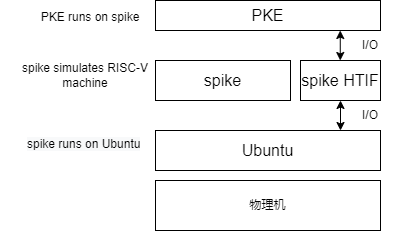
\includegraphics[width=0.6\textwidth]{images/spike_structure.png}
    \caption{模拟器环境架构}\label{模拟器环境架构} % label 用来在文中索引
\end{figure}

在硬件环境上,我们的系统是运行上PYNQ-Z2开发板上。
PYNQ-Z2开发板是Xilinx公司的一款开发板,
它具有丰富的外设资源、强大的性能。此外,它还兼容了Arduino和树莓派接口。

PYNQ-Z2搭载了FPGA系统和ARM处理器。FPGA可以烧录RISC-V CPU软核,
ARM硬核可以运行Ubuntu操作系统。我们的代理内核PKE运行在RISC-V CPU软核上,
而提供外设功能的Ubuntu则运行在ARM硬核上。
PKE和Ubuntu之间是通过riscv-fesvr通信的。
riscv-fesvr是PYNQ开发板上的重要工具,没有它,PKE就无法调用ARM上的Ubuntu I/O接口。
riscv-fesvr通过共享内存的方式,接收PKE的请求,使用ARM端的资源,并向PKE提供资源与功能。

如下图,本文给出了硬件环境的系统架构。

\begin{figure}[htbp]
    \vspace{13pt} % 调整图片与上文的垂直距离
    \centering
    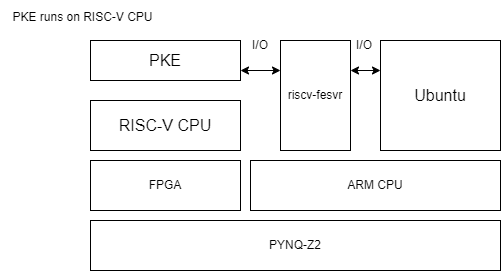
\includegraphics[width=0.6\textwidth]{images/pke_hardware_env.drawio.png}
    \caption{硬件环境架构}\label{硬件环境架构} % label 用来在文中索引
\end{figure}

\subsection{PKE移植前开发环境的优缺点}

在上一小节,本文简单介绍了PKE在移植前的开发环境。
在本小节,本文会客观分析PKE原先的物理开发环境的优点与缺点。

在原先的物理环境中,代理内核的系统是运行在PYNQ-Z2板子上的。
PYNQ-Z2拥有FPGA和ARM物理核。FPGA可以让开发者烧录RISC-V CPU软核,
然后让开发者在RISC-V CPU软核上运行PKE。
ARM硬核可以运行Ubuntu操作系统,提供I/O功能。

从不同的开发方向看。
如果开发者是在开发CPU软核,
需要快速验证FPGA上的CPU软核并进行迭代。
这种物理环境允许开发者不实现CPU涉及I/O的功能,
便于开发快速开发和验证CPU软核。

如果开发者是在开发或学习操作系统,这种开发环境反而对开发者不利。
一个原因是提供这种物理环境的开发板PYNQ-Z2价格昂贵,成本高昂。
其价格已经快要接近一台PC机的价格。
此开发板在某网购平台上的均价已达到三千余元。
这对入门级操作系统学习者购买资料学习、课程实验教学都是不利的。

另一个原因环境配置繁琐,开发者需要在PYNQ上烧录RISC-V CPU软核,
还需要在ARM核上部署Ubuntu。
除此之外,还需要在ARM核上部署riscv-fesvr,让PKE与Ubuntu通信。
这种开发环境的部署成本和学习成本是很高的,
这对于刚入门操作系统实验学习的开发者是不利的。

总而言之,PKE系统的物理环境价格昂贵、成本高昂、搭建成本高、学习成本高,
不利于学习者入门,也不利于大规模展开实验教学。
这些是PKE移植前的物理环境的痛点。
为了解决这些痛点,本文提出了将PKE移植到K210上的方案。将在下一小节阐述该方案的收益。

\subsection{PKE移植后的预期收益}

上一小节我们提到,PKE原先的物理环境有许多缺点。
这些缺点不利于学习者入门、也不利于大规模展开实验教学。
因此,我们计划将PKE移植到K210物理环境上。
PKE移植后,我们将拥有如下收益:

\begin{enumerate}
    \item 成本低廉
    
    K210板子价格低廉。
    一块不带外设的普通K210 SoC的市场价格只需要一百多元。
    与动则就要三千余元的PYNQ-Z2相比,K210的经济成本仅仅是PYNQ-Z2的三十分之一。
    这非常有利于我们开展大规模的物理环境实验教学。
    也非常有利于入门学习者购买资料进行学习。

    \item 物理环境搭建成本低
    
    在K210上,我们不再像从前在PYNQ-Z2那样烧录RISC-V CPU软核,
    也不需要在PYNQ-Z2的ARM核上加载运行Ubuntu。
    由于K210带有RISC-V 64位CPU,我们只需要在K210上烧录并运行PKE即可。
    这使得我们的物理环境搭建成本变得极低。

    \item 环境搭建学习成本低
    
    移植PKE到K210后,我们可以使用docker配置环境包、
    编写Makefile将编译与烧录流程变得自动化。
    由于不再需要像在PYNQ-Z2上烧录RISC-V CPU软核,
    也不需要在PYNQ-Z2的ARM核上加载运行Ubuntu。
    我们的环境搭建是自动化的。环境搭建的学习成本也是很低的。

\end{enumerate}


\section{移植PKE的目标与需求分析}

\begin{enumerate}

    \item 降低PKE在物理环境的开发成本
    
    移植PKE的首要目标,是降低PKE在物理环境的开发成本。
    这其中包括降低购买硬件资源的经济成本,也包括降低环境搭建的学习成本。
    这将有利于我们后续开展大规模的物理环境实验。
    也会有利于降低PKE实验的学习门槛。

    \item 用户态程序无感知
    
    PKE在移植K210的过程中,会有一定程度的内核态代码修改。
    从实验迁移的角度来看,这些内核态代码的修改应该让用户态程序无感知。
    否则,我们很有可能还要修改用户态程序,以适配修改过的PKE。
    这不仅会增加我们移植PKE的开发成本,也会增加后续实验操作者的学习成本。

    \item 减少实验操作者对移植的感知
    
    PKE移植后产生的内核态代码修改,应该尽可能地不让实验操作者感知。
    修改过后的PKE,应该对实验操作者提供与原先一致的接口,
    以降低移植对实验操作者的影响。

    \item 提高实验操作者的开发效率
    
    移植后的PKE需要能做到提高实验操作者的开发效率,
    如环境搭建更加简化、编译流程和烧录流程更加自动化、
    调试过程更加清晰化、提供给实验者的API更加易用。
    
    \item 降低PKE后续移植的成本

    经过改造后的PKE,后续移植到其他RISC-V开发板时,它的移植成本应该降低。
    也就是说,我们的移植工作应该是可复用的。
    只要是将PKE移植到其他的RISC-V开发板,我们都应该尽可能地减少对内核代码的改动。
    
\end{enumerate}

\section{移植K210前PKE的总体设计}

\subsection{系统架构}

\subsection{主要功能模块介绍}

\subsection{执行流程}

\section{移植PKE到K210的技术方案}

\section{移植K210后PKE的总体设计}

\subsection{系统架构}

\subsection{主要功能模块介绍}

\subsection{执行流程}
你好

%%
% The BIThesis Template for Bachelor Graduation Thesis
%
% 北京理工大学毕业设计(论文)第二章节 —— 使用 XeLaTeX 编译
%
% Copyright 2020-2021 BITNP
%
% This work may be distributed and/or modified under the
% conditions of the LaTeX Project Public License, either version 1.3
% of this license or (at your option) any later version.
% The latest version of this license is in
%   http://www.latex-project.org/lppl.txt
% and version 1.3 or later is part of all distributions of LaTeX
% version 2005/12/01 or later.
%
% This work has the LPPL maintenance status `maintained'.
%
% The Current Maintainer of this work is Feng Kaiyu.
% 第四章

\chapter{环境搭建}

\section{软件环境}

\subsection{编译工具链}
step1.访问sifive官网,下载riscv gcc toolchain

\href{https://www.sifive.com/software}{https://www.sifive.com/software}

step2.找到Prebuilt RISC-V GCC Toolchain。根据开发环境选择对应的版本。

\begin{figure}[htbp]
    \vspace{13pt} % 调整图片与上文的垂直距离
    \centering
    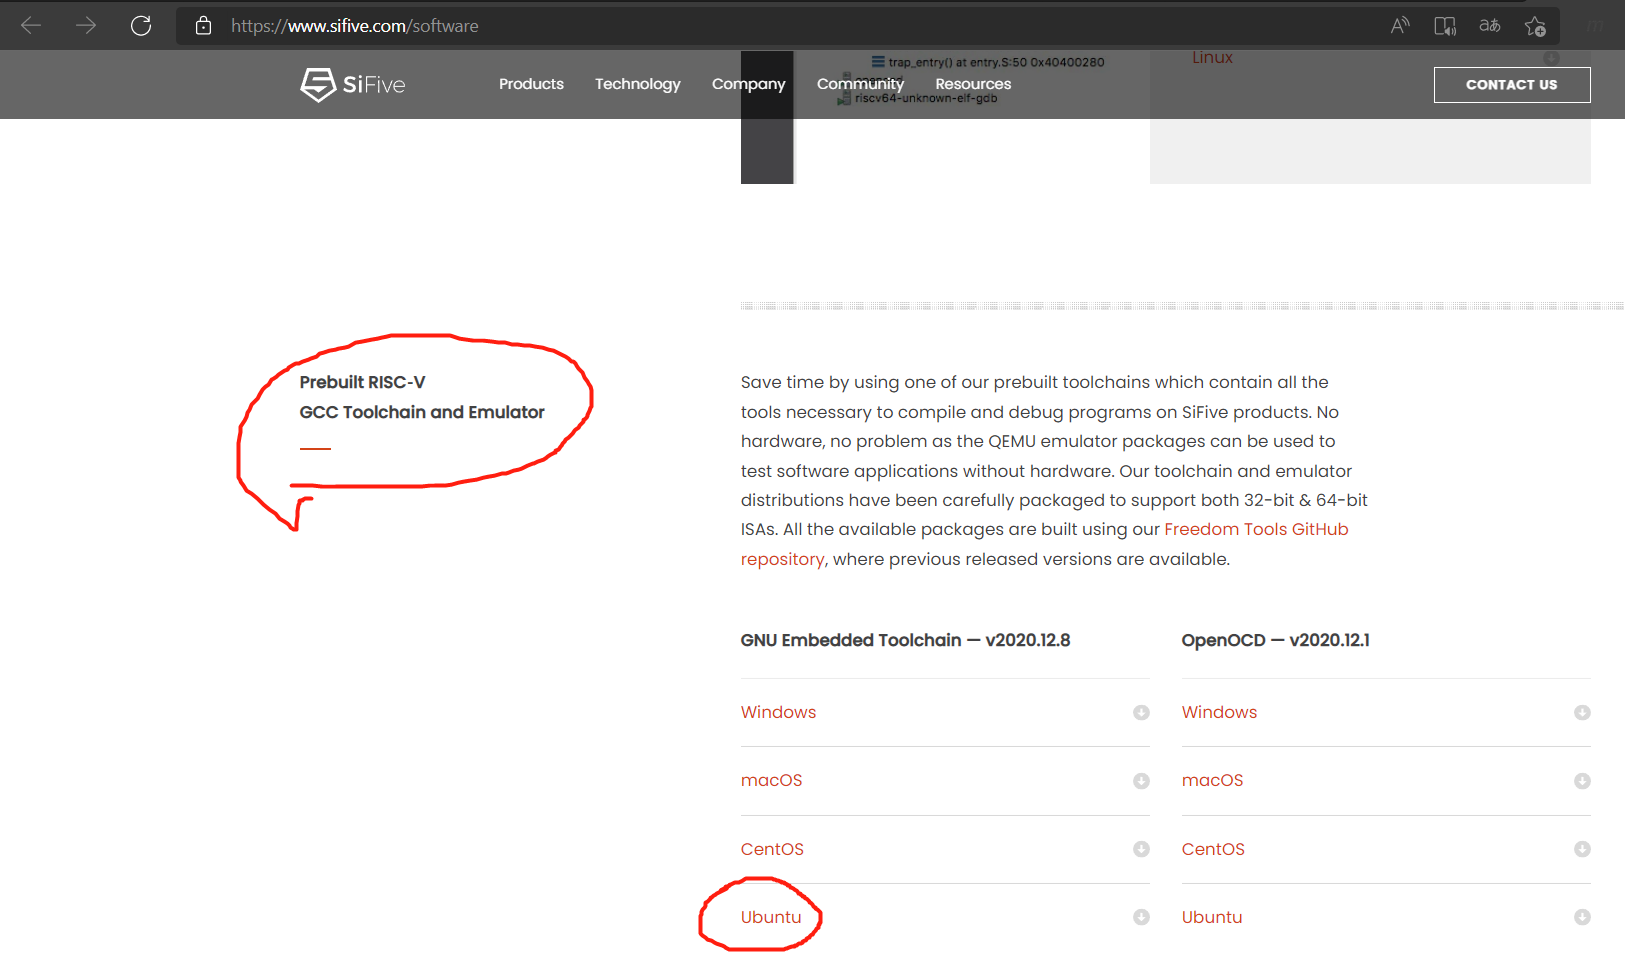
\includegraphics[width=0.9\textwidth]{images/toolchain.png}
    \caption{编译工具链列表}\label{编译工具链列表} % label 用来在文中索引
\end{figure}

step3.将下载好的tar.gz压缩包解压

\begin{lstlisting}[caption={解压命令}, label={lst:tar_command}]
    tar -zxvf $your_tar_gz
\end{lstlisting}

step4.配置环境变量。解压完成得到文件夹,进入文件夹里的bin目录,打开terminal,输入pwd获得当前路径。
复制获得的路径。将复制到的路径加入系统的PATH环境变量。

\begin{lstlisting}[caption={修改环境变量}, label={lst:change_env}]
    vim /etc/profile
    #添加以下两行到文件末尾
    export RISCV=$your_path
    export PATH=$PATH:$RISCV
\end{lstlisting}

\begin{figure}[htbp]
    \vspace{13pt} % 调整图片与上文的垂直距离
    \centering
    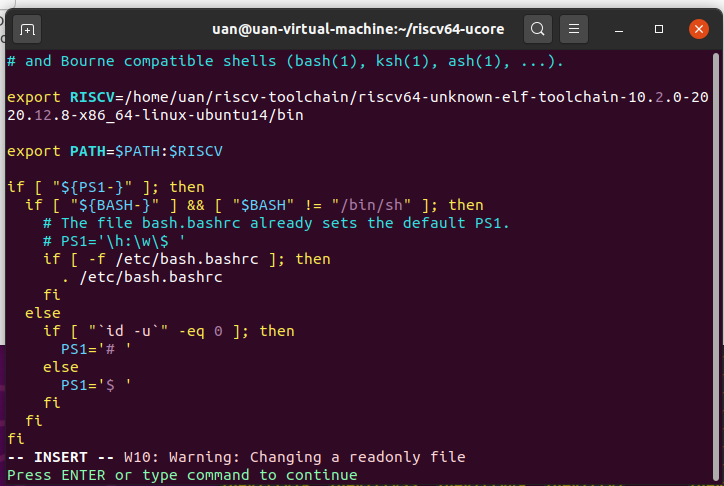
\includegraphics[width=0.9\textwidth]{images/env_path.png}
    \caption{配置环境变量}\label{配置环境变量} % label 用来在文中索引
\end{figure}

step5.加载环境变量文件

\begin{lstlisting}[caption={加载环境变量文件}, label={lst:load_env_profile}]
    source /etc/profile
\end{lstlisting}

step6.验证编译环境

在终端输入 riscv64-unknown-elf-gcc -v,如果出现以下内容,则编译环境配置成功。

\begin{lstlisting}[caption={验证编译环境}, label={lst:check_env}]
    Using built-in specs.
    ....
    gcc version 10.2.0 (SiFive GCC-Metal 10.2.0-2020.12.8) 
\end{lstlisting}

\subsection{代码准备}

step1.下载riscv64-pke-k210的代码库并查看所有分支

\begin{lstlisting}[caption={下载代码库}, label={lst:download_code}]
    git clone git@github.com:BITzga/riscv64-pke-k210.git
    git branch -a
\end{lstlisting}

step2.根据开发需求选择分支。

如下所示,k210前缀的代码分支是根据k210环境移植完成的代码。而其他普通分支则是PKE原先的代码。此时,根据开发需求使用git checkout命令选择分支即可。

\begin{lstlisting}[caption={分支列表}, label={lst:branch_list}]
    remotes/origin/k210/lab1_1_syscall
    remotes/origin/k210/lab1_2_exception
    remotes/origin/k210/lab1_3_irq
    remotes/origin/k210/lab2_1_pagetable
    remotes/origin/k210/lab2_2_allocatepage
    remotes/origin/k210/lab2_3_pagefault
    remotes/origin/k210/lab3_1_fork
    remotes/origin/k210/lab3_2_yield
    remotes/origin/k210/lab3_3_rrsched
    remotes/origin/lab1_1_syscall
    remotes/origin/lab1_2_exception
    remotes/origin/lab1_3_irq
    remotes/origin/lab2_1_pagetable
    remotes/origin/lab2_2_allocatepage
    remotes/origin/lab2_3_pagefault
    remotes/origin/lab3_1_fork
    remotes/origin/lab3_2_yield
    remotes/origin/lab3_3_rrsched
    remotes/origin/master
\end{lstlisting}

\subsection{K210环境}

\begin{itemize}
    \item Python3环境
    
    由于烧录程序和串口调试工具都是使用Python3编写的。Python是解释型语言,所以我们需要安装Python3解释器。
    除此之外我们还需要安装Python包管理工具pip。

    \begin{lstlisting}[caption={安装Python3环境}, label={lst:install_python3}]
        sudo apt-get install python3
        sudo apt-get install python3-pip
    \end{lstlisting}

    \item 烧录工具
    我们编写好的程序,经过编译,变成bin文件,还需要烧录到K210上才能运行。而烧录需要借助烧录工具,这里我们使用了\href{https://github.com/BITzga/riscv64-pke-k210/blob/master/compile_tool/kflash.py}{K-Flash}。
    \item 串口调试工具
    内核在运行时,输出信息是通过串口输出的,我们需要一个串口调试工具来接收K210上的串口信息。这里我们需要安装并使用miniterm。

    \begin{lstlisting}[caption={安装miniterm}, label={lst:install_miniterm}]
        sudo apt-get install miniterm
    \end{lstlisting}

    \item RustSBI-K210支持包
    SBI是RISC-V的规范之一,它规定了监管者二进制(Supervisor Binary Interface)接口。
    RustSBI-K210是SBI标准的一种实现,它使用Rust语言进行编写,具有性能安全的特点。
    除此之外,RustSBI-K210还对K210板子提供了特殊的支持。它还可以在K210上作为我们内核程序的Bootloader。
    我们需要使用RustSBI-K210支持包来支持内核移植,这里我们需要在烧录内核时引入RustSBI-K210支持包。

    在这里,我们可以下载到RustSBI-K210的release版本

    \href{https://github.com/rustsbi/rustsbi-k210/releases}{https://github.com/rustsbi/rustsbi-k210/releases}
    
\end{itemize}

\section{硬件环境}

\subsection{K210硬件要求}

硬件环境较为简单,我们只需要一块具有串口功能的K210板子和一根数据线即可。


% 第五章
\chapter{移植PKE的具体实现}

\section{引入RustSBI}

\subsection{SBI背景与现状}

移植K210时,PKE需要依赖SBI(Supervisor Binary Interface)提供BOOTLOADER和RUNTIME功能,所以烧录内核时需要带上SBI固件。
通过调研发现,OpenSBI与RustSBI(用Rust语言实现的SBI)均按照SBI标准实现。这两种也是业内使用最多的开源SBI。
qemu就是用了OpenSBI为RISC-V提供了环境支持。
此外,RustSBI还对K210做了特殊支持。
所以目前暂定使用RustSBI当作SBI固件,为PKE提供BOOTLOADER功能和RUNTIME运行时服务。
移植过程中我们不需要关心RustSBI的具体实现,只需要根据SBI标准调用其接口即可。

除此之外,引入SBI,可以便于内核在其他板子上运行。
当更换板子时,不需要改变内核代码,只需要更改RustSBI的支持包,获取对应硬件平台的支持包即可。
这也简化了后续内核在其他芯片的移植工作。

\subsection{RustSBI的中断和异常委托}

\subsection{RustSBI提供bootLoader功能与运行时服务}

\subsection{使用RustSBI兼容K210旧版指令集}

RustSBI在K210兼容了高版本的指令。
K210实现的RISC-V指令集是1.9.1标准的。目前最新的特权级标准已经达到1.11。
如果我们的内核代码里有用到更高级的RISC-V汇编指令,可能会在K210上无法运行。
这种情况下,就要改动内核的代码,会带来许多工作量。
因此,使用RustSBI可以使我们免去处理RISC-V汇编版本的麻烦。

\subsection{使用RustSBI兼容不同的RISC-V开发板}

\section{编译流程改造}

\subsection{编译流程改造的背景}

\subsection{内存布局改造}
由于我们引入了RustSBI,RustSBI需要占用0x80000000-0x8001FFFF的物理内存空间。所以,内核的程序入口点由此发生了变化。我们需要修改内核lds文件,更改了程序的入口点以保证内核可以正常运行。

首先,我们现在mentry.S中加入以下两行代码,用以确保\_mentry是内核的程序入口点。

\begin{lstlisting}[caption={修改内核程序入口点}, label={lst:change_kernel_entry}]
    .globl _mentry
    .section .text.prologue, "ax"
    _mentry:
\end{lstlisting}

确定了内核的程序入口点,还需要把程序入口点的地址设置为0x80020000,这需要我们对内存布局进行改造。
修改BASE\_ADDRESS,赋值为0x80020000.并设置代码段的起始地址为BASE\_ADDRESS,自此,内存布局就修改完成了。

\begin{lstlisting}[caption={修改内存布局}, label={lst:change_memory_layout}]
    OUTPUT_ARCH(riscv)
    ENTRY(_mentry)
    BASE_ADDRESS = 0x80020000;
    SECTIONS
    {
      /*--------------------------------------------------------------------*/
      /* Code and read-only segment                                         */
      /*--------------------------------------------------------------------*/
    
      /* Begining of code and text segment, starts from DRAM_BASE to be effective before enabling paging */
      . = BASE_ADDRESS;
      
      /* text: Program code section */
      .text : 
      {
        stext = .;
        *(.text.prologue);
        *(.text .stub .text.* .gnu.linkonce.t.*);
        . = ALIGN(0x1000);
        ......
       }
    
\end{lstlisting}

\subsection{Makefile改造}

由于我们需要引入RustSBI,并需要将其打包进入内核。
除此之外,还需要将内核烧录到K210,并与K210进行串口通讯。
现有的Makefile并不支持这些工作。因此,我们需要修改MakeFile。

\begin{lstlisting}[caption={修改Makefile}, label={lst:change_makefile}]
    $(KERNEL_K210_TARGET): $(KERNEL_TEMP_TARGET) $(BOOTLOADER)
    $(COPY) $(BOOTLOADER) $@
    $(V)dd if=$(KERNEL_TEMP_TARGET) of=$@ bs=128K seek=1
\end{lstlisting}

整体的编译流程为:

1.打包内核

\begin{lstlisting}[caption={打包内核}, label={lst:pack_kernel}]
    $(KERNEL_K210_TARGET): $(KERNEL_TEMP_TARGET) $(BOOTLOADER)
    $(COPY) $(BOOTLOADER) $@
     $(V)dd if=$(KERNEL_TEMP_TARGET) of=$@ bs=128K seek=1
\end{lstlisting}


以上步骤是为了把rust-sbi.bin和pke.img打包成kernel.img。
bs=128k意味着输入/输出的block大小为128k,seek=1意味着跳过第零个block进行复制操作。
也就是说,内核镜像里第零个block存放着rust-sbi.bin,第一个block才开始存放pke.img。
128k对应着十六进制0x20000,也就是二进制的0010 0000 0000 0000 0000。

我们的kernel.img放置在0x80000000处,再加上以上原因,pke的地址自然就是0x8020000。
所以,我们需要在链接脚本kernel.lds里指定内核起始地址为0x8020000,这也相当于告诉SBI这是内核的起始地址。
当SBI在行使bootloader的功能时,会跳转到0x8020000,将控制权转接给内核。

2.烧录

用数据线将K210与上位机连接,再使用kflash,指定好相关参数即可完成烧录。

\begin{lstlisting}[caption={烧录}, label={lst:burn}]
    $(PYTHON) compile_tool/kflash.py -p $(PORT) -b 1500000 $(KERNEL_K210_TARGET)
\end{lstlisting}

3.运行minitem,与K210进行串口通讯

\begin{lstlisting}[caption={运行minitem}, label={lst:run_minitem}]
    $(TERM) --eol LF --dtr 0 --rts 0 --filter direct $(PORT) 115200
\end{lstlisting}

打开miniterm,接收K210的串口打印输出。

4.总结

最小可执行内核在K210的运行流程是:
指定内核起始地址->打包完整内核镜像->
烧录到flash->引导程序加载和运行RustSBI->
RustSBI运行并跳转到内核的指定地址->
RustSBI将控制权交接给内核->内核运行

\subsection{编译自动化脚本编写}

\section{内核启动流程改造}

\subsection{内核启动流程改造前后对比}

\subsection{用户程序加载}

在原先pke的中,是通过调用spike接口,进而调用linux的文件系统接口来加载用户程序的。
而在K210上,我们没有spike的环境支持,不能直接调用spike接口。
因此,加载用户程序就需要自行实现文件系统,或者使用其他办法。

由于文件系统的实现较为繁琐,其工作量会阻塞这个移植进度。
因此,我们暂时不实现文件系统,而是采用获取用户程序地址,再加载的办法来实现这个需求。

具体的做法是:

\begin{enumerate}
    \item 将用户程序、内核和RustSBI一起编译打包到kernel.img
    \item 使用objdump命令查找到用户程序main函数的地址
    \item 得到地址以后,把地址的值赋值到内核加载用户程序处
\end{enumerate}

通过这种技术方案,我们可以用较低的开发成本实现用户程序加载。

\subsection{内核程序入口点修改}

由于RustSBI已经运行在M态,并且为我们提供了许多运行时服务。
有了RustSBI,在K210上,pke运行在M态会破坏RustSBI的设计,因此pke只需要运行在S态即可。

这样,我们就可以直接将pke的M态代码根据自身需求迁移到S态代码。
迁移完成后,需要更改内核程序入口点至S态入口

修改mentry.S文件,将call m\_start 替换成 call s\_start

\subsection{内核初始化}

\section{驱动开发}

\subsection{串口驱动}

\subsection{时钟驱动}

\section{HTIF依赖移除及接口移植}

PKE已有代码对spike提供的HTIF(Host-Target InterFace)接口存在依赖。
当PKE需要打印字符串到屏幕、访问主机上的文件或设备时会调用HTIF相关接口。
PKE通过HTIF接口调用Linux对应接口,进而实现访问外部设备的功能。

如果需要在K210上维持和原先PKE在spike模拟器一样的环境。
K210板子要同时运行PKE和Linux两个内核程序,还要提供spike模拟器类似的与Linux访问的HTIF接口。
这样的移植方案的开发成本会很高。并且收益不大。

所以移植PKE到K210时,我们需要移除PKE对HTIF的依赖,自行实现其依赖功能,编写相关代码。
这样K210只需要运行一个内核程序(PKE)即可,移植工作的开发成本会很低。

\subsection{涉及接口梳理}

\subsubsection{串口相关接口}
运行在K210上的PKE,需要使用串口接口来进行串口的访问。打印字符串到上位机。这样子才能方便我们进行实验验证,程序调试。
PKE原先并未实现串口功能,而是通过调用HTIF接口来使用串口功能。因此,我们需要自行实现串口功能。

\subsubsection{文件系统相关接口}

原先的PKE没有实现文件系统,而是通过调用HTIF接口来使用文件系统功能。
PKE在加载用户elf程序文件时,通过调用HTIF接口来访问用户程序文件,从而将用户程序加载到内存中。
最后再运行用户程序。

\subsubsection{Device Tree相关接口}

此接口的功能是用于读取设备树文件,以屏蔽SoC细节。

\subsubsection{shutdown接口}

供panic使用的接口,用于关闭设备。在内核panic时调用。PKE原先并未实现该功能,而是通过调用HTIF接口来实现。

\subsubsection{poweroff接口}

供panic使用的接口,用于关闭设备电源。在内核assert失败时使用。PKE原先并未实现该功能,而是通过调用HTIF接口来实现。

\subsubsection{定时器接口}

此接口用于PKE设置定时中断,读取时间。
PKE中是使用MMIO(memory mapping IO)来设置定时中断。
由于K210开发板此方面的资料较少,不确定K210是否支持此方式。
从减少开发成本的角度考虑,该接口使用SBI接口来实现的方案最低,可以免去查阅资料和测试的成本。
因此,该接口也需要我们进行移植。

\subsection{接口移植的技术方案及实现}

\subsubsection{串口及格式化输出实现}

由于我们已经引入了RustSBI,我们很容易实现串口输出。
我们只需要调用SBI提供的串口服务即可。

\begin{lstlisting}[language=C, caption={串口实现代码}, label={lst:serial_output} ]
    uint64 SBI_CONSOLE_PUTCHAR = 1;
    uint64 sbi_call(uint64 sbi_type, uint64 arg0, uint64 arg1, uint64 arg2) {
    uint64 ret_val;
    __asm__ volatile (
    "mv x17, %[sbi_type]\n"
    "mv x10, %[arg0]\n"
    "mv x11, %[arg1]\n"
    "mv x12, %[arg2]\n"
    "ecall\n"
    "mv %[ret_val], x10"
    : [ret_val] "=r"(ret_val)
    : [sbi_type] "r"(sbi_type), [arg0] "r"(arg0), [arg1] "r"(arg1), [arg2] "r"(arg2)
    : "memory"
    );
        return ret_val;
    }

    void sbi_console_putchar(unsigned char ch) {
        sbi_call(SBI_CONSOLE_PUTCHAR, ch, 0, 0);
    }
\end{lstlisting}

有了串口输出的方法,接下来我们需要格式化输出sprint.sprint定义在spike\_utils.c,接下来我们看看sprint的代码实现。

\begin{lstlisting}[language=C, caption={sprint实现代码}, label={lst:sprint} ]
    void sprint(char *buf, const char *fmt, ...) {
        va_list args;
        va_start(args, fmt);
        vsnprintf(buf, 1024, fmt, args);
        va_end(args);
    }
\end{lstlisting}

sprint函数的第一个参数对应了一个字符串的起始地址,第二个参数...代表可变参数。接下来我们点开vprintk的实现:

\begin{lstlisting}[language=C, caption={vprintk实现代码}, label={lst:vprintk} ]
    void vprintk(const char* s, va_list vl) {
        char out[256];
        int res = vsnprintf(out, sizeof(out), s, vl);
        //you need spike_file_init before this call
        spike_file_write(stderr, out, res < sizeof(out) ? res : sizeof(out));
    }
\end{lstlisting}

通过阅读代码发现,vsnprintf并没有将字符串真正输出到控制台。
而是根据原先的字符串和参数做字符串格式化,将最终结果保存在out数组中。

真正将字符串打印的函数调用是spike\_file\_write。
这个函数是调用了spike的接口,通过spike去调用Linux的字符串打印API。
所以我们需要在K210上实现串口输出,方案已经很明显,就是将vprintk函数中的spike\_file\_write函数替换成sbi\_console\_putchar实现的打印函数cputs。

\begin{lstlisting}[language=C, caption={vprintk改造代码}, label={lst:vprintk_dev} ]
    void vprintk(const char *s, va_list vl) {
        char out[256];
        int res = vsnprintf(out, sizeof(out), s, vl);
        cputs(out);
    }
    /* *
     * cputs- writes the string pointed by @str to stdout and
     * appends a newline character.
     * */
    int cputs(const char *str) {
        int cnt = 0;
        char c;
        while ((c = *str++) != '\0') {
            cputch(c, &cnt);
        }
        cputch('\n', &cnt);
        return cnt;
    }   
\end{lstlisting}

至此,我们完成了串口实现和格式化输出。通过在K210上验证,我们的sprint可以通过串口,在控制台上输出格式化的字符串。

\subsubsection{文件系统相关接口}

\subsubsection{Device Tree相关接口}

PKE运行在S态,设备树文件已经由M态的RustSBI读取并处理。因此PKE不需要读取和解析设备树文件。
所以,我们在移植时,只需要去除PKE读取DTB的代码即可。

\subsubsection{shutdown与poweroff接口}

内核在编码调试过程中,需要借助一些方法来判断变量值是否符合预期,如assert方法。
如果不符合预期需要打印错误信息,并且让内核panic。
那么panic在pke上是如何实现的呢?我们可以阅读pke实现panic的代码。

\begin{lstlisting}[language=C, caption={panic实现代码}, label={lst:panic} ]
    void do_panic(const char *s, ...) {
        va_list vl;
        va_start(vl, s);
        sprint(s, vl);
        shutdown(-1);
        va_end(vl);
    }
    
    void shutdown(int code) {
      sprint("System is shutting down with exit code %d.\n", code);
      frontend_syscall(HTIFSYS_exit, code, 0, 0, 0, 0, 0, 0);
      while (1)
        ;
    }    
\end{lstlisting}

通过观察我们可以发现,panic的调用链路是:

do\_panic->shutdown->frontend\_syscall

最终panic是通过frontend\_syscall调用spike提供的接口实现的。
既然是需要调用spike的HTIF,与spike的HTIF具有依赖关系,那么我们移植的时候就需要去除相关依赖,自行实现do\_panic函数。

通过观察panic和poweroff功能,很容易发现,他们都是打印报错信息,然后终止了硬件线程(hart)。
那么我们可以通过调用SBI的shutdown接口来实现这两个接口,打印报错以后以后,终止所有的hart。

\subsubsection{定时器接口}

参考uCore通过调用SBI接口来实现定时器接口。

\section{用户程序加载}
你好

\subsection{单个进程加载}
你好

\subsection{多进程支持}
你好
\chapter{代理内核实验的参考实现}

在本章节,我们将给出移植K210后的代理内核实验的参考实现。
每个实验实现的阐述结构大致相同,
先从实验的用户程序开始,描述实验的目标和预期效果。
最后我们会给出实验的参考实现代码和实现过程描述。

\section{系统调用}

\subsection{实验预期}

给定用户态应用user/app\_helloworld.c。

\begin{lstlisting}[caption={用户态应用app\_helloworld.c}, label={lst:app_helloworld}, language=C]
    #include "user_lib.h"

    int main(void) {
        printu("Hello world!\n");
        exit(0);
    }   
\end{lstlisting}

实验的目标是PKE能够加载并成功运行它。
实验预期是应用通过系统调用,成功打印出“Hello world!”,并正常退出。

\subsection{具体实现}

如上的用户态代码很简单,只有两行。第一行是用户态的打印函数printu()。
第二行是退出进程的函数exit()。
关于printu()和exit()函数的定义在user\_lib.c。
接下来我们看看这两个函数的具体实现:

\begin{lstlisting}[caption={printu与exit的实现}, label={lst:printu_exit}, language=C]
    int printu(const char *s, ...) {
        va_list vl;
        va_start(vl, s);
        char out[256];  // fixed buffer size.
        int res = vsnprintf(out, sizeof(out), s, vl);
        va_end(vl);
        const char *buf = out;
        size_t n = res < sizeof(out) ? res : sizeof(out);

        return do_user_call(SYS_user_print, (uint64) buf, n, 0, 0, 0, 0, 0);
    }

    int exit(int code) {
        return do_user_call(SYS_user_exit, code, 0, 0, 0, 0, 0, 0);
    }   
\end{lstlisting}

观察发现,printu()和exit()函数的实现都是简单处理了输入的参数,
然后就调用了do\_user\_call()函数。他们俩都是通过系统调用来获取自己所需的功能。
那么结论已经很明显,
我们只需要在PKE的内核代码中实现printu()和exit()的系统调用即可。

观察内核代码发现,printu()和exit()的系统调用都已经实现,
系统调用部分只有handle\_syscall()并未实现。该函数的功能是让用户进程的pc值增加4。
之所以增加4,是因为RISC-V的指令是32位的,32位代表着4个字节。
然后调用系统调用,最终将返回值保存在a0寄存器中。接下来我们给出它的实现代码。

\begin{lstlisting}[caption={handle\_syscall的实现}, label={lst:handle_syscall}, language=C]
static void handle_syscall(trapframe *tf) {
    tf->epc += 4;
    tf->regs.a0 = do_syscall(tf->regs.a0, tf->regs.a1,
                                tf->regs.a2, tf->regs.a3, 
                                tf->regs.a4, tf->regs.a5, 
                                tf->regs.a6, tf->regs.a7);
}
\end{lstlisting}

将实验要求实现后,我们可以在K210上运行实验代码,得到如下结果。

\begin{lstlisting}[caption={lab1实验结果}, label={lst:lab1_result}]
    [rustsbi] Version 0.1.0
    .______       __    __      _______.___________.  _______..______   __
    |   _  \     |  |  |  |    /       |           | /       ||   _  \ |  |
    |  |_)  |    |  |  |  |   |   (----`---|  |----`|   (----`|  |_)  ||  |
    |      /     |  |  |  |    \   \       |  |      \   \    |   _  < |  |
    |  |\  \----.|  `--'  |.----)   |      |  |  .----)   |   |  |_)  ||  |
    | _| `._____| \______/ |_______/       |__|  |_______/    |______/ |__|
    
    [rustsbi] Platform: K210
    [rustsbi] misa: RV64ACDFIMSU
    [rustsbi] mideleg: 0x222
    [rustsbi] medeleg: 0x1ab
    [rustsbi] Kernel entry: 0x80020000
    Enter supervisor mode...
    
    Application program entry point (virtual address): 0x00000000800206b2
    
    Switch to user mode...
    
    Hello world!
    
    User exit with code:0.
    
    System is shutting down with exit code 0.
    
    [rustsbi] todo: shutdown all harts on k210; program halt
        
\end{lstlisting}

\section{异常处理}

\subsection{实验预期}

给定用户态应用user/app\_illegal\_instruction.c

\begin{lstlisting}[caption={用户态应用app\_illegal\_instruction.c}, label={lst:app_illegal_instruction}, language=C]
    int main(void) {
        printu("Going to hack the system by running privilege instructions.\n");
        asm volatile("csrw sscratch, 0");
        exit(0);
    }
\end{lstlisting}

我们可以看到,用户态程序执行了非法指令csrw。
这个指令的执行在U模式是不被允许的,
在U模式执行这个指令会产生非法指令异常。
我们的实验预期是PKE能够捕获执行这个指令时产生的非法指令异常,
并进行简单处理。

\subsection{实验分析}

由于RustSBI-K210支持包对K210进行了兼容性的处理。
K210实现的RISC-V指令集版本是1.9.1,而最新的RISC-V指令集版本是1.11.0。
为了能让K210能够运行高版本的RISC-V指令,
该支持包捕获了高版本指令产生的异常,然后将其转换为低版本的指令。
这种机制使得我们可以在K210上运行最新版的RISC-V指令。

为了保持这种兼容性,指令异常只能由M模式的RustSBI处理,
我们不能将指令异常托管给S模式的PKE。
所以此次实验,我们没有办法在PKE中完成,
只能交给RustSBI处理。
所幸,RustSBI已经实现了非法指令的捕获与处理,
当用户程序执行非法指令时,RustSBI会捕获异常,
并且产生panic,输出panic信息。这和原来实验的预期是一致的。

此次实验不需要我们改动PKE代码,就可以得到预期效果:

\begin{lstlisting}[caption={lab2实验结果}, label={lst:app_illegal_instruction_result}]
    [rustsbi] Version 0.1.0
    .______       __    __      _______.___________.  _______..______   __
    |   _  \     |  |  |  |    /       |           | /       ||   _  \ |  |
    |  |_)  |    |  |  |  |   |   (----`---|  |----`|   (----`|  |_)  ||  |
    |      /     |  |  |  |    \   \       |  |      \   \    |   _  < |  |
    |  |\  \----.|  `--'  |.----)   |      |  |  .----)   |   |  |_)  ||  |
    | _| `._____| \______/ |_______/       |__|  |_______/    |______/ |__|
    
    [rustsbi] Platform: K210
    [rustsbi] misa: RV64ACDFIMSU
    [rustsbi] mideleg: 0x222
    [rustsbi] medeleg: 0x1ab
    [rustsbi] Kernel entry: 0x80020000
    Enter supervisor mode...
    
    Application program entry point (virtual address): 0x0000000080020788
    
    Switch to user mode...
    
    Going to hack the system by running privilege instructions.
    
    [rustsbi] panicked at 'invalid instruction, mepc: 0000000080020798, instruction: 14005073', platform/k210/src/main.rs:522:17
        
\end{lstlisting}

\section{定时器中断}

\subsection{实验预期}

给定用户态应用user/app\_long\_loop.c

\begin{lstlisting}[caption={用户态应用app\_long\_loop.c}, label={lst:app_long_loop}, language=C]
    #include "user_lib.h"

    int main(void) {
      printu("Hello world!\n");
      int i;
      for (i = 0; i < 100000000; ++i) {
        if (i % 5000000 == 0) printu("wait %d\n", i);
      }
      exit(0);
    }
\end{lstlisting}

实验操作者需要初始化时钟中断,
设置定时器中断的时间间隔,
并且编写时钟中断处理程序。
最终让用户程序执行循环的同时,
定时打印出自增的次数。

\subsection{具体实现}

\begin{lstlisting}[caption={定时器中断处理程序}, label={lst:app_timer_handler}, language=C]

    //时钟初始化部分已在kernel.c中的s_start()中完成。
    void handle_stimer_trap() {
        sprint("Ticks %d\n", ++g_ticks);
        clock_set_next_event();
    }    
\end{lstlisting}

我们的实现逻辑很简单,就是让定时器中断的次数自增,并打印输出。
然后设置下一次定时器中断的时间。

\section{虚拟地址和物理地址的转换}

\subsection{实验预期}

给定用户态应用user/app\_helloworld\_no\_lds.c

\begin{lstlisting}[caption={用户态应用app\_helloworld\_no\_lds.c}, label={lst:app_helloworld_no_lds}, language=C]
    #include "user_lib.h"
    
    int main(void) {
      printu("Hello world!\n");
      exit(0);
    }    
\end{lstlisting}

此时的用户程序是没有链接脚本文件的。
用户程序在编译和链接时并未指定好程序中符号的地址。
与此同时,PKE已经开启虚拟内存,
用户进程的物理内存空间也被映射到虚拟内存上了。

用户进程在调用printu时,它会通过ecall指令,切换到拥有更高特权级的S模式的内核,
让内核完成打印输出。需要指出的是,用户进程传入内核的地址参数是虚拟地址,
内核需要将该虚拟地址转换成物理地址才能访问字符串“Hello world!”。

所以我们的实验预期是内核成功转换用户进程传入的虚拟地址,并完成打印输出。

\subsection{具体实现}

\begin{lstlisting}[caption={虚拟地址到物理地址的转换}, label={lst:app_virt_to_phys}, language=C]
    ssize_t sys_user_print(const char* buf, size_t n) {
        //buf is an address in user space on user stack,
        //so we have to transfer it into phisical address (kernel is running in direct mapping).
        assert( current );
        char* pa = (char*)user_va_to_pa((pagetable_t)(current->pagetable), (void*)buf);
        sprint(pa);
        return 0;
    }    

    void *user_va_to_pa(pagetable_t page_dir, void *va) {
        uint64 va0 = (uint64) va;
        pte_t *PTE = page_walk(page_dir, va0, 0);
        uint64 pa = 0;
        if (PTE) {
            pa = PTE2PA(*PTE) + (va0 & ((1 << PGSHIFT) - 1));
            return (void *) pa;
        } else {
            return NULL;
        }
    }    
\end{lstlisting}

虚拟地址到物理地址的转换逻辑很简单,
首先是通过调用page\_walk()函数,查找虚拟地址的页表项。
找到页表项以后,再通过PTE2PA()函数和一些移位操作获得物理地址。

\section{基本的内存管理}

\subsection{实验预期}

给定用户态应用user/app\_naive\_malloc.c

\begin{lstlisting}[caption={用户态应用app\_naive\_malloc.c}, label={lst:app_naive_malloc}, language=C]
    #include "user_lib.h"
    
    struct my_structure {
      char c;
      int n;
    };
    
    int main(void) {
      struct my_structure* s = (struct my_structure*)naive_malloc();
      s->c = 'a';
      s->n = 1;

      printu("s: %lx, {%c %d}\n", s, s->c, s->n);
    
      naive_free(s);
      exit(0);
    }   
\end{lstlisting}

如用户程序所示,我们的PKE需要支持内存的分配和回收。
而内存的分配逻辑在PKE中已经实现好了,我们现在还需要实现内存的回收。
也就是实现naive\_free()函数。


\subsection{具体实现}

\begin{lstlisting}
    uint64 sys_user_free_page(uint64 va) {
        user_vm_unmap((pagetable_t)current->pagetable, va, PGSIZE, 1);
        return 0;
    }  
    
    void user_vm_unmap(pagetable_t page_dir, uint64 va, uint64 size, int free) {
        if (free) {
            pte_t *PTE = page_walk(page_dir, va, 0);
            if (PTE != NULL) {
                free_page(user_va_to_pa(page_dir, (void *) va));
                *PTE = *PTE & (~PTE_V);
            } else {
                sprint("PTE of free page is NULL\n");
            }
        }
    }    
\end{lstlisting}

内存回收的逻辑稍微复杂一些,
我们首先是根据根页表项与虚拟地址去调用page\_walk()函数,
得到需要回收的虚拟地址对应的页表项。
然后我们将页表项的PTE\_V位置0,这意味着此页表项将变成无效页表项。
与此同时,我们通过free\_page()函数将物理页面回收。
在这里我们只考虑一个物理页。

\section{栈空间不足与缺页异常}

\subsection{实验预期}

给定应用user/app\_sum\_sequence.c

\begin{lstlisting}[caption={用户态应用app\_sum\_sequence.c}, label={lst:app_sum_sequence}, language=C]
    #include "user_lib.h"
    #include "../util/types.h"

    uint64 sum_sequence(uint64 n) {
      if (n == 0)
        return 0;
      else
        return sum_sequence( n-1 ) + n;
    }
    
    int main(void) {
      uint64 n = 1000;
      printu("Summation of an arithmetic sequence from 0 to %ld is: %ld \n", n, sum_sequence(n) );
      exit(0);
    }
        
\end{lstlisting}

如上代码所示,
用户程序执行了一个递归求等差数列的函数,递归的层数是1000层。
显然,这么深的递归层数,很容易导致栈溢出,从而导致缺页异常。

所以我们的实验预期是PKE能够捕获缺页异常,
并且能够为用户进程的栈空间进行一定的扩容。
让该用户进程成功运行。

\subsection{具体实现}

\begin{lstlisting}[caption={handle\_page\_fault}, label={lst:handle_page_fault}, language=C]
    void handle_user_page_fault(uint64 mcause, uint64 sepc, uint64 stval) {
        sprint("handle_page_fault: %lx\n", stval);
        switch (mcause) {
            case CAUSE_STORE_PAGE_FAULT:
                if (stval < USER_STACK_TOP 
                        && (stval - USER_STACK_TOP) >= 20 * (STACK_SIZE)) {
                    user_vm_map((pagetable_t) current->pagetable,
                                    stval - stval % PGSIZE, 
                                    PGSIZE, 
                                    (uint64) alloc_page(),
                                    prot_to_type(PROT_WRITE | PROT_READ, 1));
                } else {
                    panic("handle_page_fault: stack overflow\n");
                }
                break;
            default:
                sprint("unknown page fault.\n");
                break;
        }
    }    
\end{lstlisting}

\section{创建子进程fork的实现}

\subsection{实验预期}

给定应用user/app\_naive\_fork.c

\begin{lstlisting}[caption={用户态应用app\_naive\_fork.c}, label={lst:app_naive_fork}, language=C]
    #include "../user/user_lib.h"
    #include "../util/types.h"
    
    int main(void) {
        uint64 pid = fork();
        if (pid == 0) {
            printu("Child: Hello world!\n");
        } else {
            printu("Parent: Hello world! child id %ld\n", pid);
        }
    
        exit(0);
    }
       
\end{lstlisting}

如用户代码所示,PKE需要创建一个用户进程的子进程,然后调度运行两者。

\subsection{具体实现}

如下所示,我们在kernel/process.c中补全了do\_fork()函数。

\begin{lstlisting}[caption={do\_fork}, label={lst:do_fork}, language=C]
    //                panic("You need to implement the code segment mapping of child in lab3_1.\n");
    for (int j = 0; j < parent->mapped_info[i].npages; j++) {
        map_pages(child->pagetable, 
                    parent->mapped_info[i].va + j * PGSIZE, 
                    (uint64) _etext - USER_PROGRAM_ENTRY,
                    USER_PROGRAM_ENTRY, 
                    prot_to_type(PROT_WRITE | PROT_READ | PROT_EXEC, 1));

        sprint("do_fork map code segment at pa:%lx of parent to child at va:%lx.\n",
               USER_PROGRAM_ENTRY, parent->mapped_info[i].va + j * PGSIZE);
    }    
\end{lstlisting}

\section{进程的控制权交接}

\subsection{实验预期}

给定应用user/app\_yield.c

\begin{lstlisting}[caption={用户态应用app\_yield.c}, label={lst:app_yield}, language=C]
    #include "../user/user_lib.h"
    #include "../util/types.h"
    
    int main(void) {
        uint64 pid = fork();
        uint64 rounds = 0xffff;
        if (pid == 0) {
            printu("Child: Hello world! \n");
            for (uint64 i = 0; i < rounds; ++i) {
                if (i % 10000 == 0) {
                    printu("Child running %ld \n", i);
                    yield();
                }
            }
        } else {
            printu("Parent: Hello world! \n");
            for (uint64 i = 0; i < rounds; ++i) {
                if (i % 10000 == 0) {
                    printu("Parent running %ld \n", i);
                    yield();
                }
            }
        }
    
        exit(0);
        return 0;
    }
    
\end{lstlisting}

如用户代码所示,父子进程都轮流执行了yield()函数。
yield()函数是一个可以交出进程自己的CPU执行权的函数。
yield()函数是由PKE内核实现的系统调用功能之一。

我们的实验预期是,父子进程之间的调度是可以交替的,
也就是说父子进程之间需要轮流打印出他们对应的字符串。

\subsection{具体实现}

如下,本文给出了yield()函数的实现。实现逻辑较为简单,就不再具体阐述了。

\begin{lstlisting}[caption={yield}, label={lst:yield}, language=C]
    ssize_t sys_user_yield() {
        assert(current);
        current->status = READY;
        insert_to_ready_queue(current);
        schedule();
    
        return 0;
    }    
\end{lstlisting}

\section{进程的时间片调度}

\subsection{实验预期}

给定应用user/app\_two\_long\_loops.c

\begin{lstlisting}[caption={用户态应用app\_two\_long\_loops.c}, label={lst:app_two_long_loops}, language=C]
   #include "../user/user_lib.h"
   #include "../util/types.h"
   
   int main(void) {
       uint64 pid = fork();
       uint64 rounds = 100000000;
       uint64 interval = 10000000;
       uint64 a = 0;
       if (pid == 0) {
           printu("Child: Hello world! \n");
           for (uint64 i = 0; i < rounds; ++i) {
               if (i % interval == 0) printu("Child running %ld \n", i);
           }
       } else {
           printu("Parent: Hello world! \n");
           for (uint64 i = 0; i < rounds; ++i) {
               if (i % interval == 0) printu("Parent running %ld \n", i);
           }
       }
   
       exit(0);
       return 0;
   }
       
\end{lstlisting}

如上代码所示,
我们的用户父子进程不再主动调用yield()函数交出自己的CPU执行权。
而是由PKE内核利用时间片轮询的方式来调度父子进程,
定时地切换父子进程的执行权。

所以我们的实验预期是,完成PKE内核中时间片调度进程的实现,
并让父子进程交替执行。

\subsection{具体实现}

\begin{lstlisting}[caption={时间片调度}, label={lst:time_slice}, language=C]
    void smode_trap_handler(void) {
        assert(current);
        current->trapframe->epc = read_csr(sepc);
        uint64 cause = read_csr(scause);
    
        switch (cause) {
            case CAUSE_STIMER_S_TRAP:
                handle_stimer_trap();
                rrsched();
                break;
            default:
                //......省略展示此部分代码......
        }
        switch_to(current);
    }

    void rrsched() {
        assert(current);
        if (current->tick_count < TIME_SLICE_LEN) {
            current->tick_count++;
        } else {
            current->tick_count = 0;
            current->status = READY;
            insert_to_ready_queue(current);
            schedule();
        }
    }    
\end{lstlisting}

时间片调度进程的实现,是通过设置定时器中断,
当S模式的PKE拦截到定时器中断时,
就会执行中断处理程序,处理程序其中就包括了进程的切换。

\section{实验资料的管理}

在我们移植实验的过程中,我们使用了git来管理PKE移植的代码,
并且将移植后的代码放置在了GitHub仓库中。GitHub仓库的链接如下:

\href{https://github.com/BITzga/riscv64-pke-k210}{https://github.com/BITzga/riscv64-pke-k210}。

此代码库包含18个主要分支,其中有9个分支是PKE移植前的代码分支,
这9个分支的代码保持不变,没有受到修改,是移植前的基础分支,
也可以供我们进行移植前后的代码比较。

此外还有另外9个k210前缀的分支。他们是移植后的代码分支,均已通过功能测试
,都可以被烧录和运行在K210上, 并且可以达到实验预期效果。

\begin{lstlisting}[caption={分支列表}, label={lst:branch_list_1}]
    remotes/origin/k210/lab1_1_syscall
    remotes/origin/k210/lab1_2_exception
    remotes/origin/k210/lab1_3_irq
    remotes/origin/k210/lab2_1_pagetable
    remotes/origin/k210/lab2_2_allocatepage
    remotes/origin/k210/lab2_3_pagefault
    remotes/origin/k210/lab3_1_fork
    remotes/origin/k210/lab3_2_yield
    remotes/origin/k210/lab3_3_rrsched
    remotes/origin/lab1_1_syscall
    remotes/origin/lab1_2_exception
    remotes/origin/lab1_3_irq
    remotes/origin/lab2_1_pagetable
    remotes/origin/lab2_2_allocatepage
    remotes/origin/lab2_3_pagefault
    remotes/origin/lab3_1_fork
    remotes/origin/lab3_2_yield
    remotes/origin/lab3_3_rrsched
\end{lstlisting}

此外,我们在移植开发工作完成以后,
还编写了相关的实验指导书,并放置在了gitbook上。
由于时间关系,我们的实验指导书并不是特别完善,
后续我们将对其进行补充和完善。
这里我们先给出实验指导书的gitbook链接:

\href{https://1621184422.gitbook.io/pke-k210-tutorial}{https://1621184422.gitbook.io/pke-k210-tutorial}
% 结论:在结论相应的 TeX 文件处进行结论部分的撰写
%%
% The BIThesis Template for Bachelor Graduation Thesis
%
% 北京理工大学毕业设计(论文)结论 —— 使用 XeLaTeX 编译
%
% Copyright 2020-2021 BITNP
%
% This work may be distributed and/or modified under the
% conditions of the LaTeX Project Public License, either version 1.3
% of this license or (at your option) any later version.
% The latest version of this license is in
%   http://www.latex-project.org/lppl.txt
% and version 1.3 or later is part of all distributions of LaTeX
% version 2005/12/01 or later.
%
% This work has the LPPL maintenance status `maintained'.
%
% The Current Maintainer of this work is Feng Kaiyu.
%
% Compile with: xelatex -> biber -> xelatex -> xelatex

\unnumchapter{结~~~~论}
\renewcommand{\thechapter}{结论}

\ctexset{
  section/number = \arabic{section}
}

% 结论部分尽量不使用 \subsection 二级标题,只使用 \section 一级标题

% 这里插入一个参考文献,仅作参考
本文结论……。\cite{李成智2004飞行之梦}

\textcolor{blue}{结论作为毕业设计(论文)正文的最后部分单独排写,但不加章号。结论是对整个论文主要结果的总结。在结论中应明确指出本研究的创新点,对其应用前景和社会、经济价值等加以预测和评价,并指出今后进一步在本研究方向进行研究工作的展望与设想。结论部分的撰写应简明扼要,突出创新性。阅后删除此段。}

\textcolor{blue}{结论正文样式与文章正文相同:宋体、小四;行距:22 磅;间距段前段后均为 0 行。阅后删除此段。}

% 参考文献:如无特殊需要,参考文献相应的 TeX 文件无需改动,添加参考文献请使用 BibTeX 的格式
%   添加至 misc/ref.bib 中,并在正文的相应位置使用 \cite{xxx} 的格式引用参考文献
%%
% The BIThesis Template for Bachelor Graduation Thesis
%
% 北京理工大学毕业设计(论文)参考文献 —— 使用 XeLaTeX 编译
%
% Copyright 2020-2021 BITNP
%
% This work may be distributed and/or modified under the
% conditions of the LaTeX Project Public License, either version 1.3
% of this license or (at your option) any later version.
% The latest version of this license is in
%   http://www.latex-project.org/lppl.txt
% and version 1.3 or later is part of all distributions of LaTeX
% version 2005/12/01 or later.
%
% This work has the LPPL maintenance status `maintained'.
%
% The Current Maintainer of this work is Feng Kaiyu.
%
% Compile with: xelatex -> biber -> xelatex -> xelatex
%
% 如无特殊需要,本页面无需更改

% 参考文献开始
\unnumchapter{参考文献}
\renewcommand{\thechapter}{参考文献}

% 设置参考文献字号为 5 号
\renewcommand*{\bibfont}{\zihao{5}}
% 设置参考文献各个项目之间的垂直距离为 0
\setlength{\bibitemsep}{0ex}
\setlength{\bibnamesep}{0ex}
\setlength{\bibinitsep}{0ex}
% 设置单倍行距
\renewcommand{\baselinestretch}{1.2}
% 设置参考文献顺序标签 `[1]` 与文献内容 `作者. 文献标题...` 的间距
\setlength{\biblabelsep}{0.5mm}
% 设置参考文献后文缩进为 0(与 Word 模板保持一致)
\renewcommand{\itemcmd}{
  \addvspace{\bibitemsep} % 恢复 \bibitemsep 的作用
  \mkgbnumlabel{\printfield{labelnumber}}
  \hspace{\biblabelsep}}
% 删除默认的「参考文献 / Reference」标题,使用上面定义的 section 标题

% \printbibliography [type=article,heading=none] 

% \printbibliography [keyword={book},heading=none] 

% \printbibliography [type=book,heading=none] 

% \printbibliography [type=inproceedings,heading=none] 

% \printbibliography [type=inbook,heading=none] 

% \printbibliography [keyword={thesis},heading=none] 

% \printbibliography [keyword={techreport},heading=none] 

% \printbibliography [type=patent,heading=none] 

% \printbibliography [keyword={standard},heading=none] 

% \printbibliography [keyword={newspaper},heading=none] 

% \printbibliography [keyword={online},heading=none] 

% 在使用时,请删除/注释上方示例内容,并启用下方语句以输出所有的参考文献
\printbibliography[heading=none]

% 附录:在附录相应的 TeX 文件处进行附录部分的撰写
%%
% The BIThesis Template for Bachelor Graduation Thesis
%
% 北京理工大学毕业设计(论文)附录 —— 使用 XeLaTeX 编译
%
% Copyright 2020-2021 BITNP
%
% This work may be distributed and/or modified under the
% conditions of the LaTeX Project Public License, either version 1.3
% of this license or (at your option) any later version.
% The latest version of this license is in
%   http://www.latex-project.org/lppl.txt
% and version 1.3 or later is part of all distributions of LaTeX
% version 2005/12/01 or later.
%
% This work has the LPPL maintenance status `maintained'.
%
% The Current Maintainer of this work is Feng Kaiyu.
%
% Compile with: xelatex -> biber -> xelatex -> xelatex

\unnumchapter{附~~~~录}
\renewcommand{\thechapter}{附录}

% 设置附录编号格式
\ctexset{
  section/number = 附录\Alph{section}
}

附录相关内容…

% 这里示范一下添加多个附录的方法:

\section{\LaTeX 环境的安装}
\LaTeX 环境的安装。

\section{BIThesis 使用说明}
BIThesis 使用说明。

\textcolor{blue}{附录是毕业设计(论文)主体的补充项目,为了体现整篇文章的完整性,写入正文又可能有损于论文的条理性、逻辑性和精炼性,这些材料可以写入附录段,但对于每一篇文章并不是必须的。附录依次用大写正体英文字母 A、B、C……编序号,如附录 A、附录 B。阅后删除此段。}

\textcolor{blue}{附录正文样式与文章正文相同:宋体、小四;行距:22 磅;间距段前段后均为 0 行。阅后删除此段。}

% 致谢:在致谢相应的 TeX 文件处进行致谢部分的撰写
%%
% The BIThesis Template for Bachelor Graduation Thesis
%
% 北京理工大学毕业设计(论文)致谢 —— 使用 XeLaTeX 编译
%
% Copyright 2020-2021 BITNP
%
% This work may be distributed and/or modified under the
% conditions of the LaTeX Project Public License, either version 1.3
% of this license or (at your option) any later version.
% The latest version of this license is in
%   http://www.latex-project.org/lppl.txt
% and version 1.3 or later is part of all distributions of LaTeX
% version 2005/12/01 or later.
%
% This work has the LPPL maintenance status `maintained'.
%
% The Current Maintainer of this work is Feng Kaiyu.
%
% Compile with: xelatex -> biber -> xelatex -> xelatex

\unnumchapter{致~~~~谢}
\renewcommand{\thechapter}{致谢}

\ctexset{
  section/number = \arabic{section}
}

% 致谢部分尽量不使用 \subsection 二级标题,只使用 \section 一级标题

值此论文完成之际,首先向我的导师表示感谢……



\end{document}
